\noindent \textcolor{ubuntu_orange}{Nie}, nie potrzebujesz programu antywirusowego na Linuksie.\\
\textcolor{ubuntu_orange}{Tak}, istnieją wirusy na Linuksa.\\
\textcolor{ubuntu_orange}{Tak}, istnieje bardzo dużo programów antywirusowych dla Linuksa.\\
\textcolor{ubuntu_orange}{Nie}, nie potzebujesz ich, gdyż i tak nic na świecie nie zabezpieczy cię przed tobą samym.

Z wirami na Linuksa jest jak z Yeti --- są ślady, ale nikt nie widział włochacza. W praktyce szkodliwe oprogramowanie na Linuksa istnieje, ale jako wektor infekcji wykorzystuje dziury w wtyczkach do przeglądarek (Flash, Java, PDF) i przed tym żaden antywirus cię nie zabezpieczy (dotyczy to każdego systemu operacyjnego). Tu powinieneś winić producentów tychże wtyczek, czyli kolejno Oracle, Adobe i znów Adobe.

Drugim wektorem ataku jest użytkownik komputera, czyli właśnie Ty. Złośliwe oprogramowanie wykorzystuje socjotechniki aby przekonać użytkownikaPlik do uruchomienia programu z uprawnieniami administratora systemu. Na to żaden program antywirusowy nie pomoże. Żaden program antywirusowy nie zabezpieczy też przed wirusami, które nie zostały jeszcze odkryte (zasada ta dotyczky każdego systemu operacyjnego).

Konstrukcja systemu Linux sprawia, że niebywale trudno jest programowi samodzielnie zdobyć kontrolę nad systemem (fachowo się to nazywa ,,rozszerzeniem uprawnień''). Nawet jeżeli pojawi się program potrafiący dokonać takich rzeczy, łatki uszczelniające system trafiają do komputerów domowych w ciągu doby od odkrycia zagrożenia.

Każdy liczący się program antywirusowy ma swoją wersję działającą na Linuksie, jednakże jest to oprogramowanie przeznaczone do działania na serwerach pocztowych oraz w dużych siecieach korporacyjnych. Te antywirusy służą do wykrywania i unieszkodliwiania wirusów przeznaczonych na systemy z rodziny Windows.

\subsubsection{ClamAV}
\begin{wrapfigure}[8]{R}{0.5\textwidth}
	\vspace{-10pt}
	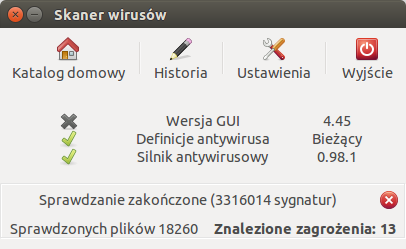
\includegraphics[width=\linewidth]{images/programy_clam.png}
\end{wrapfigure}

Jeżeli korzystasz tylko i wyłączenie z systemu Linuks (jakim jest Ubuntu) to nie potrzebujesz programu antywirusowego. Jednakże, jeżeli masz jeszcze zainstalowany obok system Windows to czasem możesz chcieć przeskanować jego partycję lub sprawdzić czy bezpiecznie jest uruchomić danego pendriva na systemie Windows.

Aby zainstalować antywirus \textcolor{ubuntu_orange}{ClamAV} wraz z nakładką graficzną wyszukaj w Centrum oprogramowania Ubuntu ,,Clamtk'' lub zainstaluj ten pakiet z wiersza poleceń:
\begin{lstlisting}[language=bash]
sudo apt-get install clamtk
\end{lstlisting}

Obsługa programu ClamTk jest bardzo prosta. Kliknij na przycisk \textcolor{ubuntu_orange}{Katalog domowy} aby rozpocząć skanowanie swojego katalogu. Po paru minutach otrzymasz raport. Clam wyszukuje nie tylko wirusy, ale też teoretycznie szkodliwe i niepożądane pliki. Jak zawsze w przypadku pracy z programem antywirusowym należy uważać na jego raporty i nie kasować jak popadnie wszystkiego co pokazuje.

Na obrazu widać, że po skanowaniu katalogu domowego autora tego Przewodnika antywirus wykrył 13 zagrożeń. Na tą listę złożyły się dwa pliki z wirusami celowo tam umieszczonymi oraz 11 wpisów w katalogu profilu przeglądarki Firefox, rozpoznane jako elementy szpiegujące.

\subsubsection{Dodatkowe opcje skanowania}
W menu \menu{Skanuj} mamy dostępne dodatkowe opcje skanowania:
\begin{itemize}
\item \textcolor{ubuntu_orange}{Plik} --- skanuje wskazany plik.
\item \textcolor{ubuntu_orange}{Katalog} --- skanuje wszystkie pliki we wskazanym katalogu bez podkatalogów.
\item \textcolor{ubuntu_orange}{Skanowanie rekursywne} --- skanuje wszystkie pliki we wskazanym katalogu wraz ze wszystkimi podkatalogami.
\item \textcolor{ubuntu_orange}{Katalog domowy (szybko)} --- skanuje katalog domowy, bez podkatalogów.
\item \textcolor{ubuntu_orange}{Katalog domowy (rekursywnie)} --- skanuje katalog domowy wraz z podkatalogami
\item \textcolor{ubuntu_orange}{Urzadzenie} --- skanuje podłączone do komputera urzadzenia wymienny (pendrivy, dyski zewnętrzne).
\end{itemize}

Aby przeskanować cały komputer wybierz \menu{Skanuj>{Skanowanie rekursywne}} i wskaż główny \textcolor{ubuntu_orange}{System plików} (/). Aby mieć pewność, ze wszystko zostało sprawdzone uruchom ClamTk jako administrator:
\begin{lstlisting}[language=bash]
sudo clamtk
\end{lstlisting}